\textbf{Diseño de la Cuña}

Para el diseño de la cuña se utiliza la norma ANSI B17.1-1967, la cual menciona que para ejes de hasta 6.5 pulgadas de diámetro, se utilizó una cuña cuadrada. Para determinar las dimensiones se utiliza la siguiente tabla:
 (Figura \ref{fg:Tamaños Cuña}). 

%\newpage

			
El tamaño de cuña para un eje de 1.5 pulgadas es de 3/8 pulgadas.

\begin{center}
	$W = \frac{3}{8} in = 9.52 mm$
\end{center}

El análisis para la cuña se realiza debido a las fallas potenciales que pueden tener al transmitir potencia, que son por corte y falla a la compresión.

Calculando la fuerza de tangencial $F_t$ que actúa sobre la cuña (Figura \ref{fg:Fuerza_T}). 

\begin{figure}[h]
    \centering
        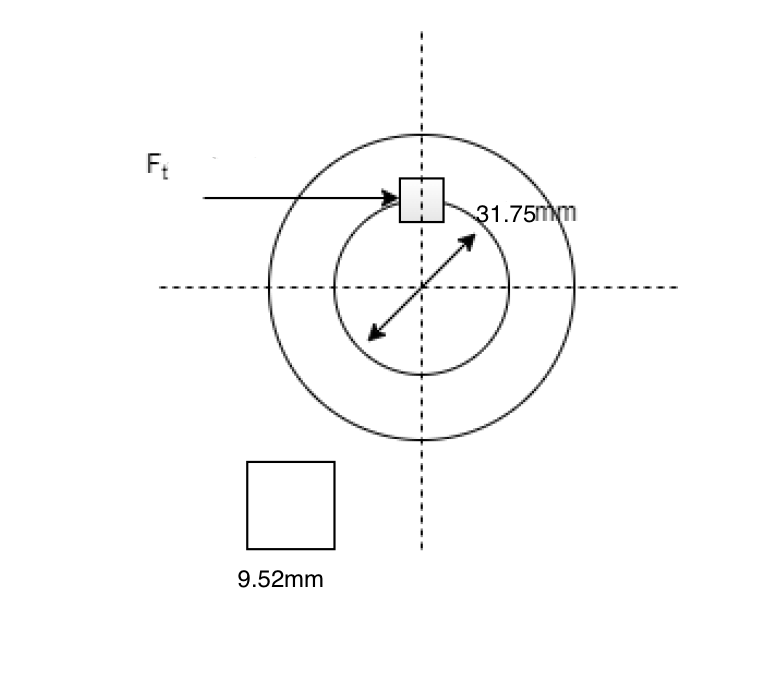
\includegraphics[scale=0.6]{images/Capitulo 4/s5/Fuerza Tangencia.png}
        \caption{Fuerza tangencial aplicada a la cuña}\cite{Mott}
    \label{fg:Fuerza_T}
\end{figure}
 

\begin{center}
	$F_t = \frac{2M_t}{d}$
\end{center}

Sustituyendo los valores previamente calculados, se tiene:

\begin{center}
	$F_t = \frac{2*40 Nm}{0.03175 m}$\\
	$F_t = 2519.68 N$\\
	$F_t \approx 2520 N$
\end{center}


En los diseños se puede igualar el esfuerzo cortante $S_y$ y el esfuerzo de diseño al cortante, para la teoría de falla por esfuerzo cortante máximo\cite{Mott}: 

\begin{center}
	$\tau_d = \frac{0.5*S_y}{N}$
\end{center}

Para aplicaciones industriales típicas, el libro \cite{Mott} recomienda $N=3$.

Si la cuña esta hecha del mismo material que el eje, acero SAE 1045, se tiene que:

\begin{center}
	$\tau_d = \frac{0.5*530.2 MPa}{3}$\\
	$\tau_d = 88.36 MPa$\\
	$\tau_d  \approx 88.5 MPa$
\end{center}

Si el esfuerzo cortante es:

\begin{center}
	$\tau = \frac{F}{A_s}$\\
	$\tau = \frac{F}{W*L}$
\end{center}

Para determinar la longitud mínima, por esfuerzo cortante, se despeja $L$ , por lo que se obtiene:

\begin{center}
	$L = \frac{F}{W*\tau}$\\
	$L = \frac{2520 N}{0.00952 m * 88.5 MPa}$\\
	$L = 2.98 mm$ \\
	$L \approx 3 mm$
\end{center}


Cálculo por aplastamiento:

\begin{center}
	$\sigma_d = \frac{\sigma_r}{N}$ \\
	$\sigma_d = \frac{630.2 MPa}{3}$ \\
	$\sigma_d \approx 210 MPa$
\end{center}

Sabiendo que el esfuerzo por aplastamiento es:

\begin{center}
	$\sigma = \frac{2*F}{H*L}$
\end{center}

Despejando $L$ se obtienes que: 
\begin{center}
	$L = \frac{2*F}{H*\sigma} = \frac{2*2520 N}{0.00952 m * 210 MPa}$
 \end{center}
 \begin{center}
	$L = 2.52 mm$ \\
	$L \approx 3 mm$
\end{center}

La cual es una longitud bastante pequeña, por lo que se propuso utilizar una con la longitud del ancho de la polea seleccionada. 
